\section{Introduction}

In this experiment we want to use the universal gas equation \cite{gas}
\begin{equation}
	\displaystyle PV=nRT
	\label{eq::gas}
\end{equation} were $P$ is the pressure, $V$ the volume, $n$ the number of particles, $R$ universal gas constant and $T$ the temperature, to determine the lowest limit of the so called thermodynamic Celsius temperature scale.
At this lowest point of temperature the enthalpy and entropy of a cooled ideal gas reaches its minimum values.
By definition this point is the zero point of the SI base unit of temperature Kelvin, which is defined as follows \cite{kelvin}:
\begin{itemize}
	\item The kelvin, symbol K, is the SI unit of thermodynamic temperature. It is defined
	by taking the fixed numerical value of the Boltzmann constant $k$ to be
	$1.380 649 \times 10^{-23}$ when expressed in the unit \si{\J}$\si{\K}^{-1}$, which is equal to $\si{\kg}$ $\si{\m}^2$ $\si{\s}^{-2}$ $\si{\K}^{-1}$,
	where the kilogram, metre and second are defined in terms of $h$, $c$ and $\Delta vC_s$.
\end{itemize}
 
In the process to find this coldest temperature possible in the absolute temperature, we use a glass bulb filled with a known gas, a pressure sensor and two well known temperatures to measure and calculate the zero point. 
Once the pressure and temperature of the gas in the glass bulb is known, all kinds of temperatures can be measured with the change of pressure in the sealed glass bulb.
To show this the temperature of liquid nitrogen is measured at the end of the experiment.
%\begin{figure}[Ht]
%	\centering
%	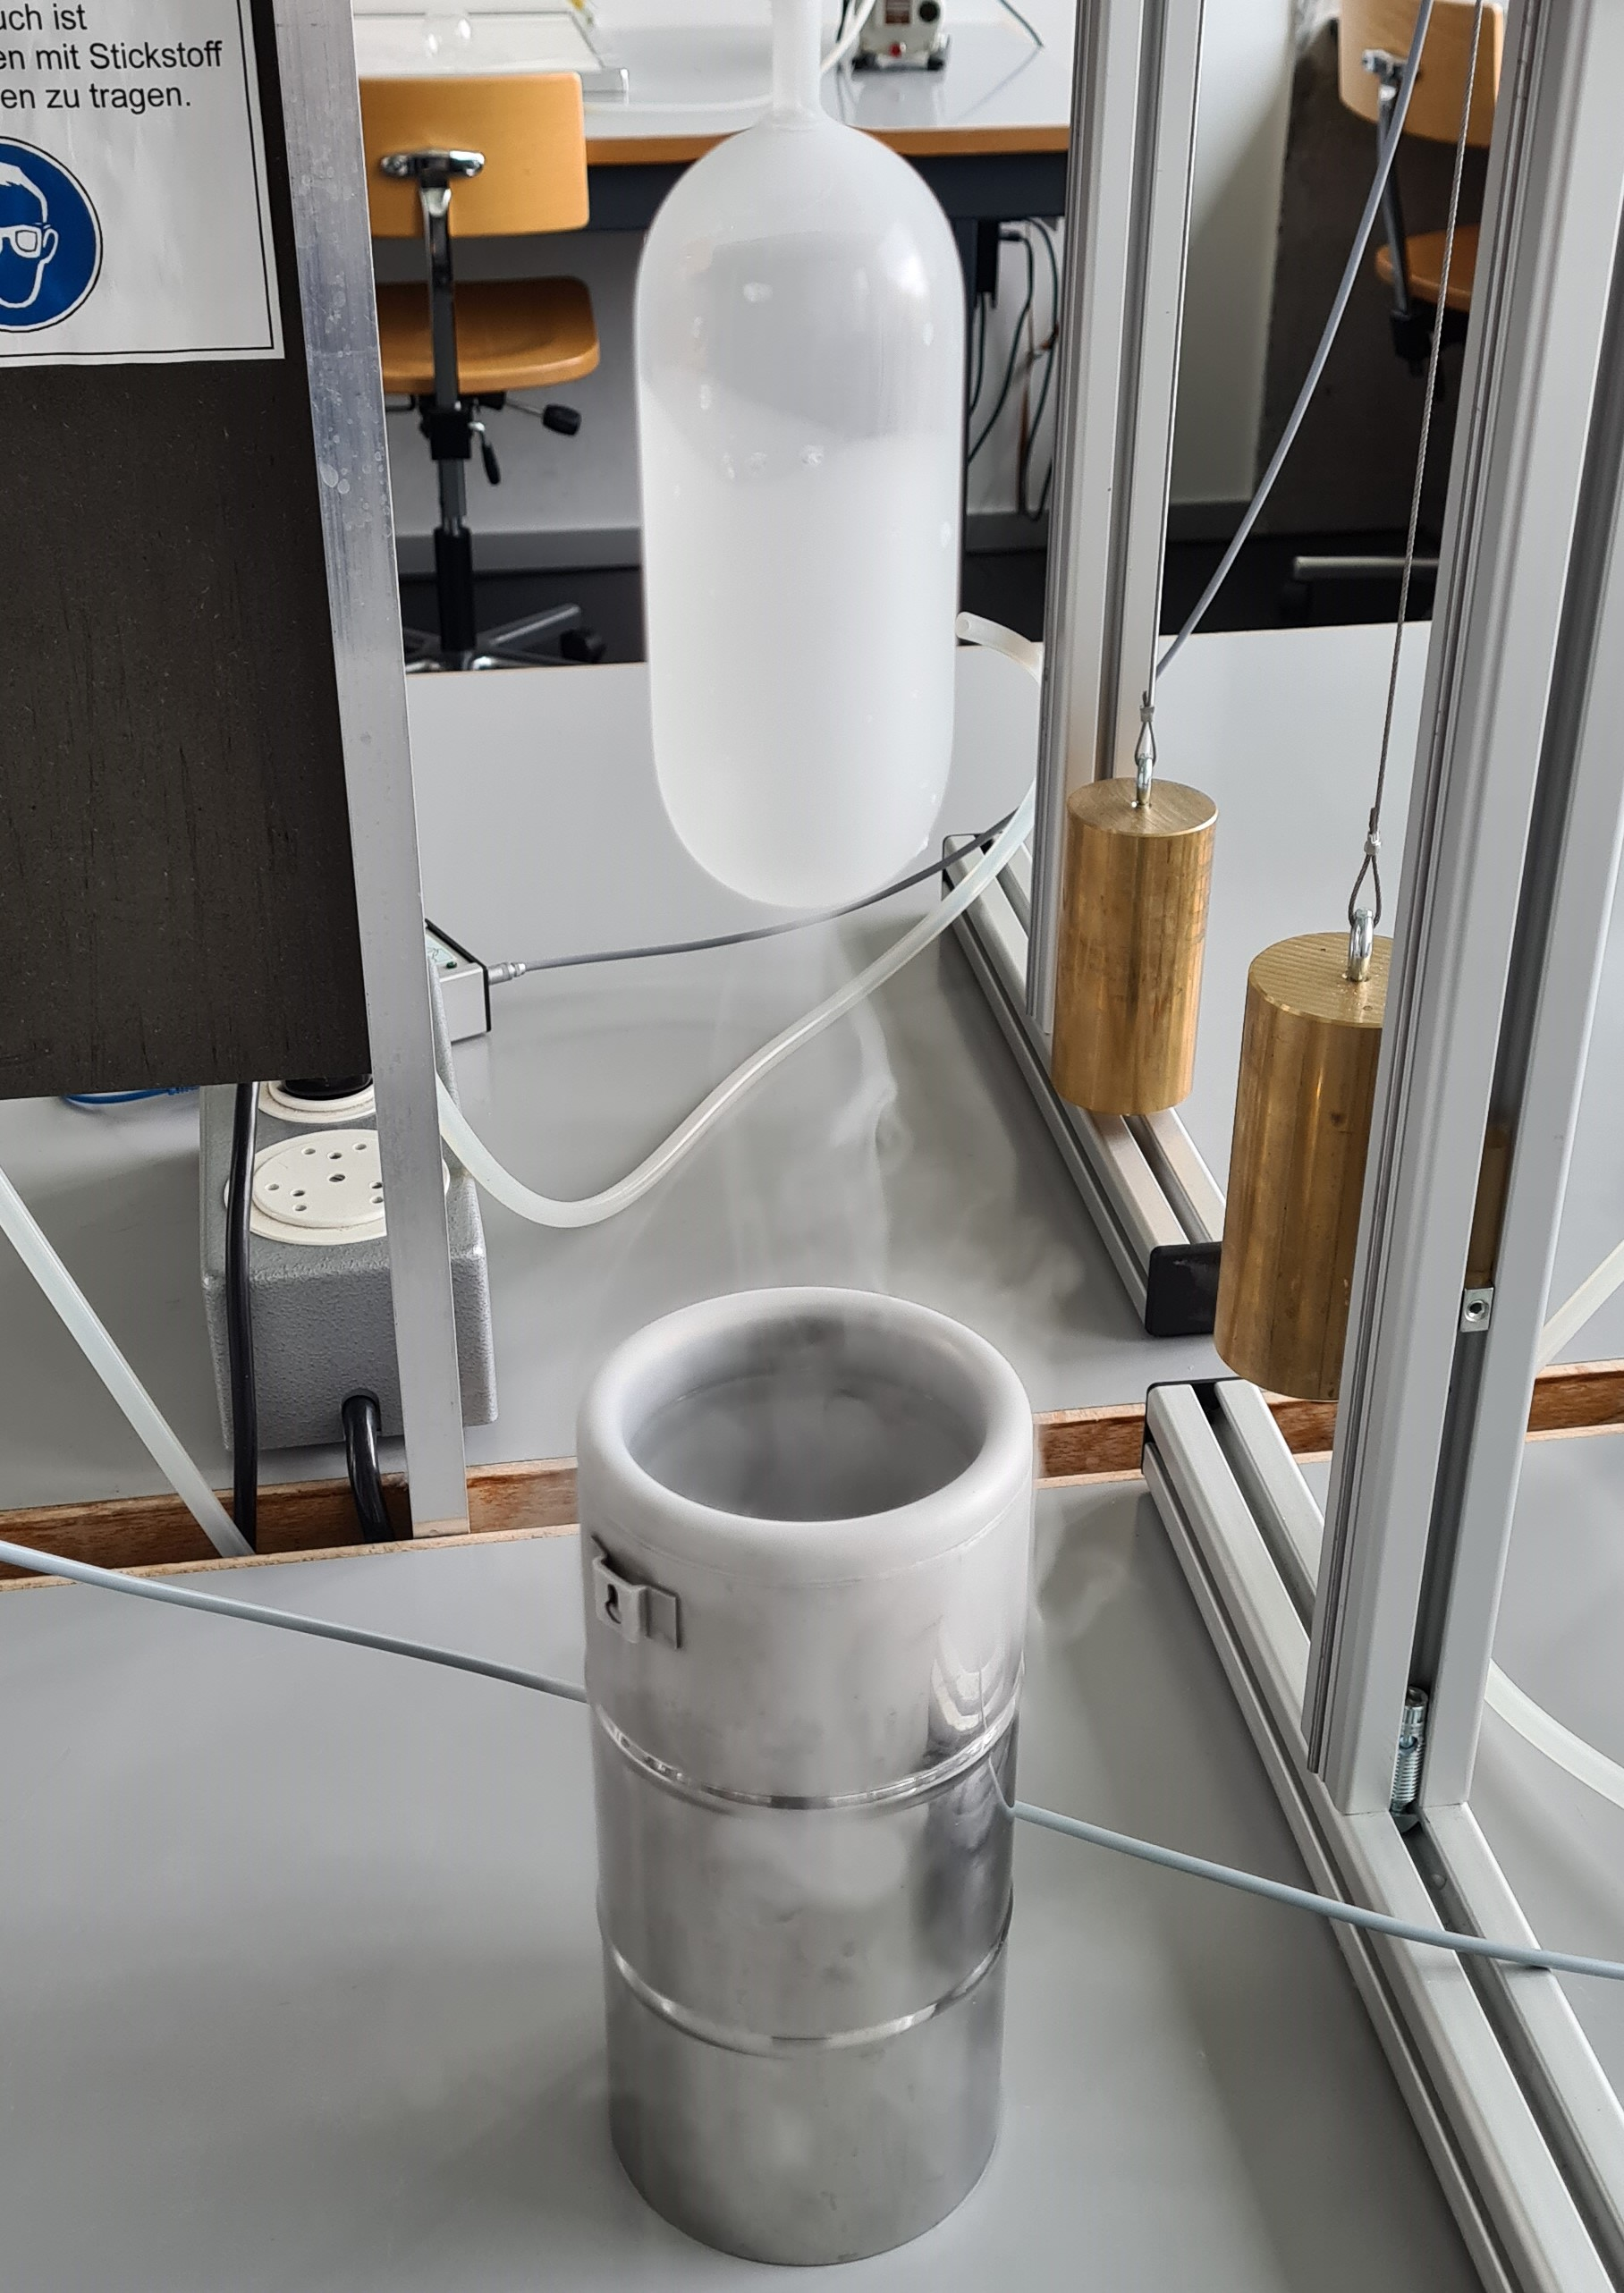
\includegraphics[width=0.5\textwidth]{sections/images/liquid.jpg}
%	\caption{Sealed glass bulb filled with helium after being put in liquid nitrogen to measure the temperature of liquid nitrogen.}
%\end{figure}
